\customchapter[January 12, 2023]{Lecture 4: DFA Acceptance}

\section{Walk in DFA}

\begin{definition}{Trap State}
    A state $q$ is a trap state iff $ \bbD(q, \bbE) = q $ for all $\bbE \in \bbE$
\end{definition}

\begin{example}
    $ \bbM = ( \{q_0, q_1, q_2\} , \{a, b\} , \bbD, q_0, \{q_1\} ) $. $L(M) = \{a^nb : n \geq 0\} $
\end{example}

\begin{figure}[!h]
    \centering
    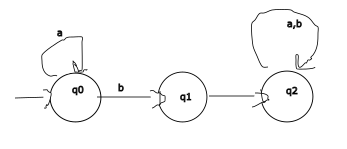
\includegraphics[width=0.5\textwidth]{figures/lec04_01.png}
    \caption{DFA}
\end{figure}

Here $q_2$ is a trap state.

\begin{theorem}{}
    Let $\bbM$ be a DFA and let $G_m$ be its graphical representation. Then for every $q_i \in Q$ and $w \in \Sigma^{+}$ we have $D^{+}(q_i, w) = q_j$ iff there is a walk from $q_i$ to $q_j$ with label $w$.
\end{theorem}

\begin{proof}
    We will use mathematical induction on the length of w.\\
    \textbf{Base case:} $w = a$. Then $D^{+}(q_i, a) = q_j$ iff there is a edge from $q_i$ to $q_j$ with label $a$. \\
    \textbf{Inductive step:} Assume for all $\left| u \right| = n < m$, if $D^{+}(q_i, u) = q_k$ then there is a walk form $q_i$ to $q_j$ with label $u$. \\ 
    Now if $w \in \Sigma^{+}$, with $\left| w \right| = n+1 = m$, say $w = ua$. \\ 
    Then $D^{+}(q_i, w) = D^{+}(D^{+}(q_i, v), a) = D^{+}(q_k, a) = q_j \implies$ there is a walk from $q_i$ to $q_j$ with label $w$. \\

    \textbf{Backward direction:} Assume for all $\left| u \right| = n < m$, if there is a walk from $q_i$ to $q_j$ with label $u$ then $D^{+}(q_i, u) = q_j$. \\
    $\square$   
\end{proof}

\textbf{\underline{Remark}}: If there is a walk from $q_i$ to $q_j$ with label $w$, then $D^{+}(q_i, w) = q_j$

\section{DFA Acceptance}

\begin{definition}{}
    A DFA accepts a string $w$ iff $w$ is accepted by $\bbM$.
\end{definition}

\begin{definition}{Regular Language}
    A language L is called regular iff there is a DFA $\bbM$ such that $L(M) = L$.
\end{definition}

\begin{example}
    Find a DFA for the language $L = \{abw : w \in \{a, b\} \}$.
\end{example}

\begin{figure}[!h]
    \centering
    
\includegraphics[width=0.5\textwidth]{figures/default.png}
    \caption{Solution to the above example}
\end{figure}

\begin{example}
    Show that the language $L = \{awa : w \in \{a, b\}^{+} \}$ is regular.
\end{example}

\begin{figure}[!h]
    \centering
    
\includegraphics[width=0.5\textwidth]{figures/default.png}
    \caption{Solution to the above example}
\end{figure}

$\oint$ How to prove that a language is not regular?

\begin{definition}{Concatanation of two languages}
    
\end{definition}